
\subsubsection{Medidor de distância a Laser}

Durante o processo de metalização o 3D scanner estará desligado, pois o tempo de
varedura não o torna prático para obter informações em tempo real. Assim o
sistema estaria funcionando em \textit{loop} aberto, o que gera receios com
relação à segurança. A fim de evitar tais riscos é desejável alguma
realimentação para o sistema sobre sua posição. Essa realimentação será
realizada pelo uso de um medidor de distância a Laser, a ser posicionado próximo
à pistola de metalização, com o intuito de aferir a distância da pistola até a
pá em tempo real.

\begin{figure}[h!]
\centering
	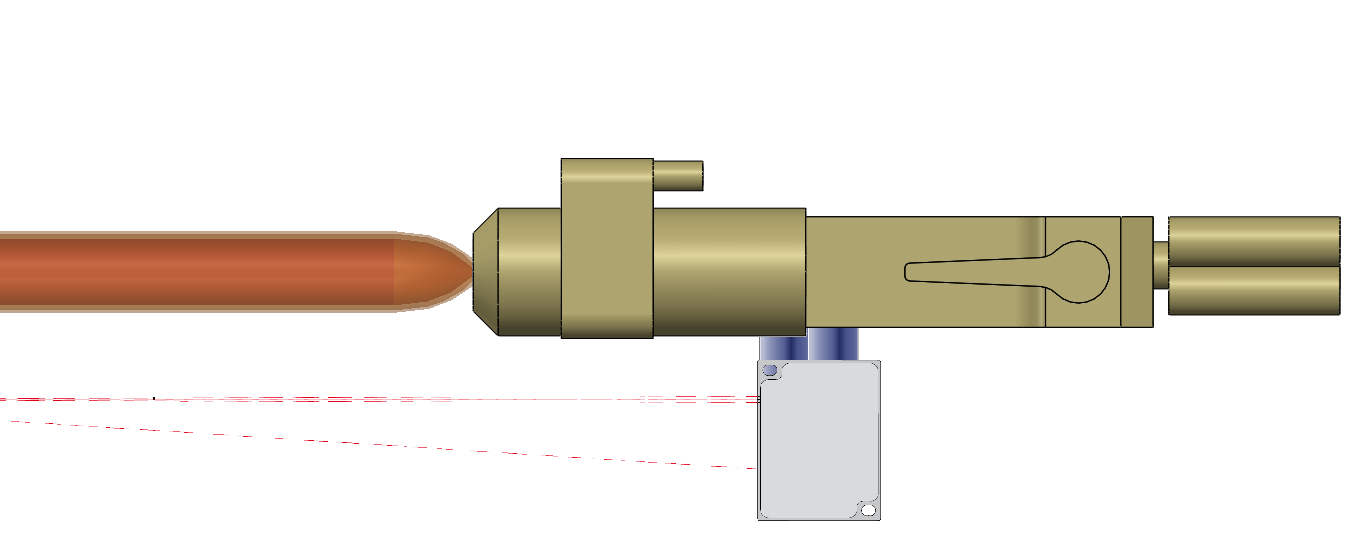
\includegraphics[width=0.9\columnwidth]{figs/3dsensors/senso_laser_pistola}
	\caption{Ilustração da posição do medidor de distância, em cinza, na pistola de
	metalização.}
	\label{fig::laser}
\end{figure}


Para a escolha de medidor compatível foram analisadas as seguintes variáveis:

\paragraph{Temperatura}
A temperatura da superfície pode influenciar na precisão do sensor devido à
radiação de corpo negro. Caso essa radiação térmica atinja níveis relevantes na
faixa de frequência do Laser utilizado ocorre degradação da qualidade de
reposta do sensor. Análises de campo identificaram que, apesar da alta
temperatura da chama de metalização, a pá da turbina não chega a emitir níveis
preocupantes de radiação na faixa do vermelho ($670 nm$), onde operam os Lasers
padrões. Para casos de exceção existem Laser que trabalham em regiões do
azul/violeta.

Por outro lado a temperatura do ambiente também influencia o sensor, que não
costuma ter alta resistência à temperatura, ficando algo em torno do $50^oC$.
Para evitar que o calor da chama seja recebido diretamente pelo sensor,
aumentando a temperatura ambiente na região, ele deve ser posicionado na pistola
com uma distância de segurança da chama (figura \ref{fig::laser}).

\paragraph{Distância de operação}
A metalização ocorre com a pistola entre 23cm e 24cm de distância da pá. Somado
a isso temos a distância do sensor à chama para então sabermos a distância da
pá ao sensor. Considerando que a pistola possui em torno de 30cm de comprimento,
a faixa de operação de distâncias do sensor deverá incluir 40-50cm. Para termos
essa região no centro da faixa de operação, ela deverá iniciar em 20-25cm e
trabalhar até 80-100cm.

\paragraph{Poeira e Umidade}
A alta umidade ambiente dentro do aro câmara, e em todo circuito hidráulico,
impõe mais um requisto sobre o equipamento. Além disso, o pó residual da
aplicação da metalização pode ser danoso ao sensor. Um isolamento apropriado
para o sensor pode ser encontrado segundo a padronização IP69K.

\paragraph{Precisão}
Como a tolerância está na ordem de milímetros ( a distância do sensor à pá deve
se manter em uma faixa de $\pm 5mm $ entre 23cm e 24cm ), logo é desejável que o
sensor possua precisão de $1mm$ ou menor.

\paragraph{Peso}
Considerando a carga máxima no punho do robô de 10kg, e a massa da pistola de
8,5kg e aplicando as restrições dinâmicas ( para manter a velocidade
desejada em todos os pontos ) conclui-se que o medido deve ter uma massa
inferior a 1kg.
